\chapter{Indicadores de Desempenho}
\label{indicadores}

Os Indicadores de desempenho também conhecidos como KPIs, da sigla em inglês Key Performance Indicators, são métricas que quantificam a performance das organizações nas mais diversas áreas, de acordo com seus objetivos e metas. Eles são utilizados para monitorar os resultados da empresa e servem como referência para o processo de tomada de decisão e a criação de estratégias de melhoria. 

Segundo Branco Filho \cite{branco2006indicadores}, somente os indicadores permitem uma quantificação e acompanhamento dos processos, eliminando a subjetividade e favorecendo as correções necessárias. Ou seja, os indicadores são dados chave para a tomada de decisão. Este capítulo apresentará os principais indicadores de desenmpenho da Manutenção e suas aplicações.

\section{Indicadores da Manutenção}
\label{SIM}

A manutenção, como a produtividade e a qualidade, por exemplo, possui diversos indicadores para sua gestão. Neste trabalho serão abordados os tradicionalmente usados com base no Documento Nacional \lq\lq A situação da Manutençã no Brasil \rq\rq realizada pela ABRAMAN (tabela~\ref{Principais indicadores de desempenho utilizados}). Estes indicadores guardam uma correlação positiva com o desempenho e a segurança na empresa, todavia estes ao serem empregados devem ser individualizados para a função específica que se deseja controlar \cite{martorell1999}.

\graphicspath{{figuras/}}	
\begin{table}[H]
\centering
\caption{Indicadores da função manutenção tradicionalmente usados no Brasil \textbf{Fonte: ABRAMAN - Associação Brasileira de Manutenção, 2009}}
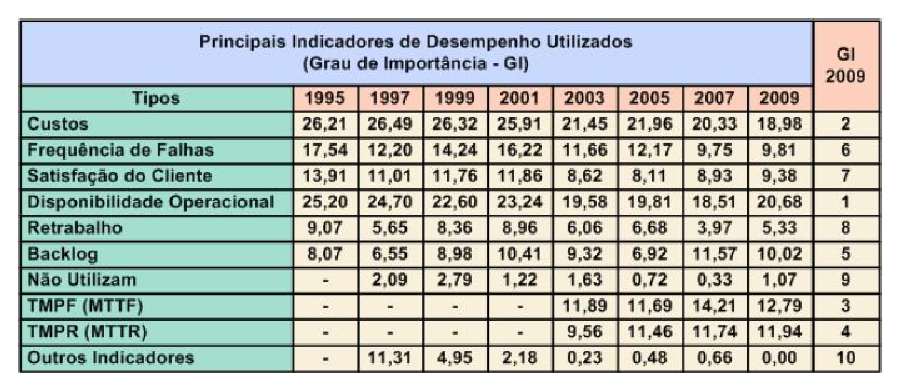
\includegraphics[width=0.8\textwidth]{PrincipaisIndicadores.eps}
\label{Principais indicadores de desempenho utilizados}
\end{table}

Qualquer que seja a forma que tomam os indicadores, os valores obtidos sobre eficiência, produtividade, segurança e disponibilidade, tem dois propósitos principais: decidir sobre o destino dos recursos e avaliar o desempenho do sistema depois que os recursos foram usados \cite{lofsten1998}. Assim, a ferramenta portadora dos indicadores permite identificar os desvios no desempenho dos equipamentos, e o controle que integra o laço de retro alimentação, que todo sistema de gestão bem implementado deve possuir. 

Segundo Martorell, \cite{martorell1999}, o primeiro passo para o desenvolvimento e implantação de KPIs deve ser a elaboração de um \lq\lq panorama \rq\rq conceitual" para a avaliação da eficácia das tarefas que estão sendo executadas em qualquer setor de uma organização, seja ele a produção, o controle de estoque, os recursos humanos ou a manutenção, por exemplo. O desenvolvimento desse panorama conceitual inicia-se com a coleta de informações básicas disponivéis nas fontes principais como o Sistema de Gerenciamento da Produção, Sistema de Informações da Manutenção e outras fontes importantes, se houver.

No caso da função Manutenção, Martorell forneceu orientações em um esquemático conceitual para a implementação do Sistema de Indicadores da Manutenção (SIM) evidenciado na figura~\ref{Sistemas de Indicadores da Manutencao}, por meio da correlação dos objetivos da produção e os objetivos da manutenção.

\graphicspath{{figuras/}}
\begin{figure}[H]
\centering
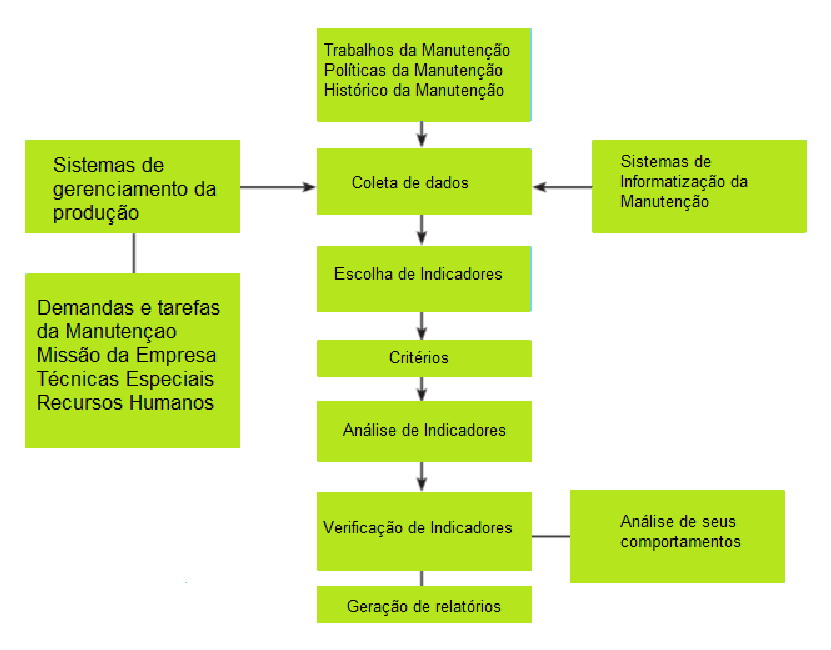
\includegraphics[width=1\textwidth]{Sistemas_de_Indicadores_da_Manuten_o.eps}
\caption{Sistemas de Indicadores da Função Manutenção.\textbf{Fonte: Autor. Adaptado de: Martorell at al:1996.}}
\label{Sistemas de Indicadores da Manutencao}
\end{figure}

O proxímo passo consiste na definição de indicadores de desempenho, propriamente ditos, os quais estão intrínsecamente relacionados com os dados operacionais, com as fases de programação e execução das tarefas, e com a contribuição para o desempenho organizacional. No caso da função Manutenção, as informações operacionais são imprescindíveis para a implantação do SIM devido sua natureza, que conforme \cite{martorell1999}, carecem ser utilizadas em conjunto com as atividades operacionais, e com os processos usuais dos setores próprios da organização. Na prática os indicadores de desempenho da manutenção são avaliados sob diferentes aspectos e abrangem dados a cerca dos equipamentos, a partir do seu histórico e nível de criticidade na planta, além de dados a cerca da eficiência da mão de obra empregada e dos programas de manutenção desenvolvidos, do nível de estoque, do custo das atividades e etc.

Na etapa de desenvolvimento e implementação do SIM, também cabe a formulação de um panorama conceitual conforme ilustrou \cite{muchiri2011development} na figura~\ref{Desempenho da funcao manutencao}, o que facilita sua avaliação sob diferentes visões identificando elementos chaves e processos que dirigem a função manutenção para a entrega de resultados exigidos pelas metas de produção. O panorama conceitual ilustrado resguarda a correlação das metas da função manutenção com a produção e os objetivos organizacionais e, assim, direciona os trabalhos da manutenção para a consecução dos objetivos de melhoria contínua dos equipamentos de produção e, consequentemente do sistema produtivo.

\graphicspath{{figuras/}}
\begin{figure}[H]
\centering
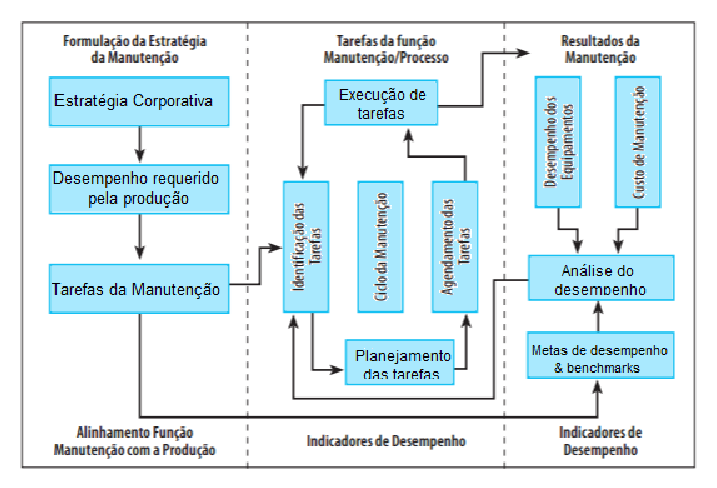
\includegraphics[width=1\textwidth]{desempenho_da_funcao_manutencao.eps}
\caption{Panorama conceitual para a análise da performance da função manutenção. \textbf{Fonte: Autor. Adaptado de Muchiri et al: 2011}}
\label{Desempenho da funcao manutencao}
\end{figure}

O panorama conceitual da Figura~\ref{Desempenho da funcao manutencao}, apresenta três partes fundamentais, a saber: A formulação da estratégia da manutenção, as tarefas/processos da função manutenção e os resultados da manutenção, e revela que o controle de qualquer sistema depende da definição de indicadores de resultados apropriados, conforme o interesse do gestor. No entanto, os indicadores devem acompanhar o desempenho da manutenção nos seus processos principais e não em aspectos particulares, para permitirem uma visão geral da condição da manutenção.

A tabela~\ref{Indicadores de desempenho} mostra os principais indicadores e índices de desempenho normalmente utizados na avaliação da performance da função manutenção \cite{branco2006indicadores}.

\graphicspath{{figuras/}}	
\begin{table}[H]
\centering
\caption{Indicadores de Desempenho. \textbf{Fonte: Branco Filho: 2006}}
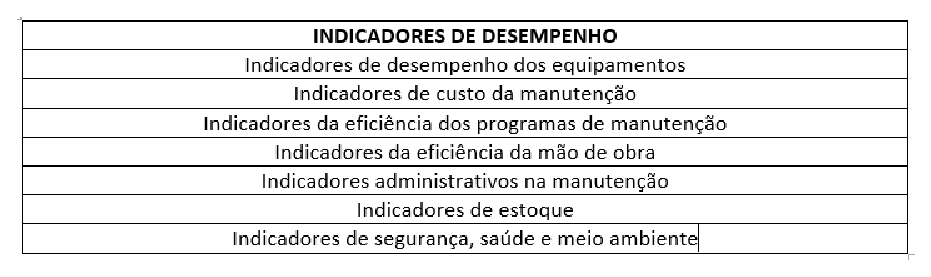
\includegraphics[width=0.8\textwidth]{IndicadoresBrancoFilho.eps}
\label{Indicadores de desempenho}
\end{table}

Sugere-se que os indicadores de desempenho, como os descritos na tabela~\ref{Indicadores de desempenho}, devem ser avaliados em blocos onde subconjuntos são analisados separadamente de acordo com seu significado e utilidade. De modo que haja ao menos três subconjutos, separados em 1) Aqueles que monitoram o desempenho da manutenção nos níveis mais baixos, como os do ciclo de vida de um equipamento 2) Aqueles que impactam o sistema de execução das manutenções e 3) Aqueles que impactam a política global da manutenções na organização voltadas a segurança, ao custo e ao desempenho \cite{de2012indicadores}, conforme tabela~\ref{Niveis de indicadores de desempenho}.

\graphicspath{{figuras/}}
\begin{table}[H]
\centering
\caption{Níveis de Indicadores de Desempenho. \textbf{Fonte: Autor}}
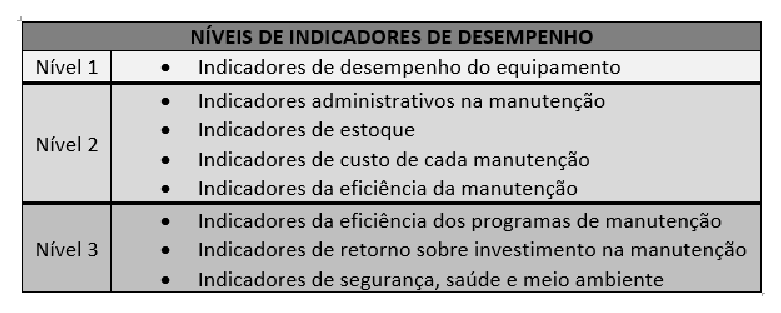
\includegraphics[width=0.8\textwidth]{niveisdeindicadores.eps}
\label{Niveis de indicadores de desempenho}
\end{table}

A forma de avaliação e o número de indicadores que serão utilizados pela organização depende fortemente do ramo de negócio e da política empresarial de manutenção que se pretende adotar. Contudo friza-se o mencionado por Xavier \cite{xavier2007indicadores} \lq\lq é melhor ter poucos indicadores importantes e acompanhá-los bem \rq\rq.

\subsection{Indicadores do equipamento}
\label{nivel 1}

Em relação aos indicadores que monitoram o desempenho da manutenção dos equipamentos baseados nas características de seus ciclos de vida (nível 1), os principais são:

\begin{itemize}
	\item R(t)- Confiabilidade;
	\item TMF - Tempo Médio de Falhas ou Mean Time of Failures;
	\item TMEF - Tempo Médio entre Falhas ou Mean Time Between Failures;
	\item TMR - Tempo Médio entre Reparos ou Mean Time Between Repair;
	\item A(t) - Disponibilidade;
	\end{itemize}

Esses indicadores medem atributos bem básicos do sistema. A primeira dessas medidas é a \textbf{confiabilidade - R(t)}. A definição convencional de confiabilidade, representa a probabilidade de que um item, um equipamento ou um sistema esteja funcionando continuamente em um intervalo de tempo \textbf{[0,t]}, ou ainda que esteja em condições de trabalho após um determinado período de funcionamento \cite{tavares1999administraccao}. 

Perto de confiabilidade estão os indicadores \textbf{Tempo Médio de Falhas (TMF)},  e \textbf{Tempo Médio Entre Falhas (TMEF)}. O primeiro é o tempo médio que o sistema opera até acontecer uma falha, enquanto o segundo é o tempo médio entre duas falhas consecutivas. A diferença entre as duas  é o tempo necessário para reparar o sistema depois da primeira falha. Estipulando Tempo Médio de Reparo (TMR):

\begin{equation}
\label{eqn01}
	\mathbf{TMEF} = \mathbf{TMF} + \mathbf{TMR} 
\end{equation}

O indicador \textbf{Tempo Médio de Reparo (TMR)} nos aponta o tempo que a equipe de manutenção demanda para reparar e disponibilizar a máquina ou equipamento para o sistema produtivo. Nesse período estão todas as ações envolvidas no reparo, sejam elas da equipe de compras, de laboratório ou qualquer outra equipe de trabalho \cite{ZEN2008}.

Outro indicador importante deste nível é a \textbf{Disponibilidade}, representada por \textbf{A(t)}, é definida como a fração média de tempo sobre o intervalo \textbf{[0,t]} que o sistema está funcionando, em outras palavras, a Disponibilidade representa a probabilidade de em um dado momento um equipamento esteja em funcionamento normal ou produção e é interpretada como a probabilidade de que o sistema estará operante em um período de tempo aleatório, e só é significativo em sistemas que incluem reparo de componentes com defeito. Pode se calcular a disponibilidade usando as seguintes equações:

\begin{equation}
\label{eqn02}
	\mathbf{A} = \mathbf{\frac{TMF}{TMEF}} = \mathbf{\frac{TMF}{TMF + TMR}}
\end{equation}
Uma medida relacionada é Ap(t), que é a probabilidade do sistema operar em um determinado instante \textbf{t}.

O uso do indicador Disponibilidade é apropriado para aplicações em que performance contínua não é vital mas onde seria caro ter o sistema fora por um período significativo de tempo. É possível que um sistema de baixa confiabilidade tenha uma alta disponibilidade, por exemplo, um sistema que cai toda hora, mas se recupera em um segundo.

\subsection{Indicadores do sistema de execução das manutenções}
\label{nivel 2}

No tocante aos indicadores que impactam o sistema de execução das manutenções (nível 2), os principais são:

\begin{itemize}
	\item IMF - Custo total de manutenção por faturamento bruto;
	\item IMBA - Custo total de manutenção por ativo imobilizado;
	\item MP - Cumprimento dos planos de manutenção preventiva e preditiva;
	\end{itemize}

O acompanhamento dos custo de manutenção, são um dos principais indicadores que a atividade de manutenção deve observar, representando a somatória básica de todo recurso financeiro utilizado pelo setor, compreendendo: custos de intervenção de manutenção (recursos materiais, sobressalentes e mão de obra), custos próprios (internos) da equipe de manutenção, tais como administração, treinamento, etc. Além destes, a atividade de manutenção deve estimar os custos de perdas de produção (se houver), e o custo da perda de oportunidade pela falta do produto se houver demanda. Normalmente as empresas acompanham apenas os custos de intervenção, mas devem no mínimo acompanhar também os custos próprios \cite{ZEN2008}.

Bem assim, os indicadores \textbf{custo total de manutenção por faturamento bruto (IMF)} e \textbf{custo total de manutenção por ativo imobilizado (IMBA)} são calculados da seguinte formula: 

\begin{equation}
\label{eqn03}
	\mathbf{IMF} = \mathbf{\frac{\textrm{ custo total de manutencao}}{\textrm{faturamento bruto}}} 
\end{equation}

\begin{equation}
\label{eqn04}
	\mathbf{IMBA} = \mathbf{\frac{\textrm{ custo total de manutencao}}{\textrm{ valor base do ativo sem depreciacao}}} 
\end{equation}

Perceba aqui que o indicador \textbf{IMF} usa em seu cálculo a variável faturamento bruto, o que pode gerar uma falsa percepção por sua inaplicabilidade dentro de organizações governamentais, porém podemos utilizar este mesmo indicador para o caso de instituições que não possuem um faturamento o valor de seu orçamento anual. E assim aferir o quanto está se gastando em manutenção em termos percentuais, por exemplo. Este indicador se torna importante a medida que comparamos seu valor com o usualmente adotado por outras organizações ou empresas do setor da empresa que está sendo monitorada.

Ao lado dos indicadores de custo, estão os índices que acompanham o processo de planejamento e execução das manutenções preventivas e preditivas, os quais podem ser visualizados por meio de um diagrama de Venn ~\ref{Diagrama de Venn da programacao}, representando os conjuntos de ações programadas e realizadas, no universo de planejamento, em um dado periodo de tempo. 

\graphicspath{{figuras/}}
\begin{figure}[H]
\centering
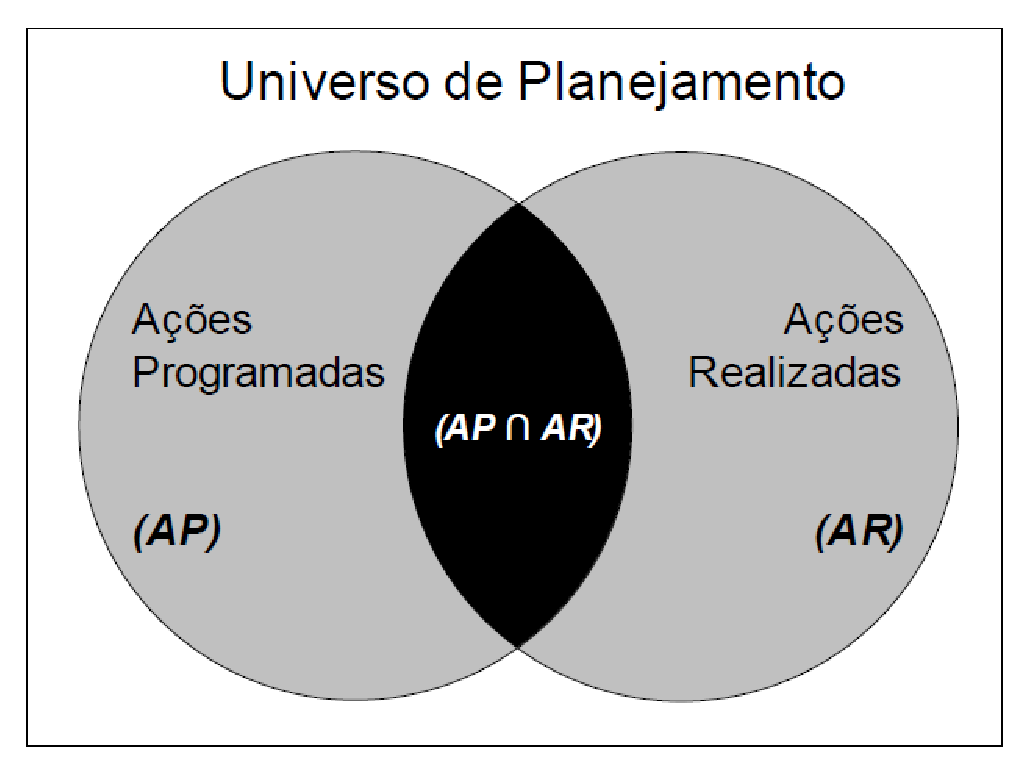
\includegraphics[width=0.6\textwidth]{Diagrama_de_Venn.eps}
\caption{Diagrama de Venn do cumprimento dos planos de manutenção preventiva e preditiva \textbf{Fonte:\cite{de2006indicadores}}}
\label{Diagrama de Venn da programacao}
\end{figure}

Em uma situação ideal, os conjuntos {AP} e {AR} seriam idênticos, havendo perfeita correlação das ações executadas com as ações planejadas. Na prática, as imperfeições do processo, de origem internas à programação e execução, ou externas, oriundas do meio ambiente ou de agentes fora do controle do planejador, geram diferenças entre estes conjuntos, reduzindo a qualidade do planejamento. Para medir a eficiência do processo de programação, será útil associar um universo de referência ao conjunto união dos itens programados e executados, { AP U AR } \cite{de2006indicadores}.

Para avaliação destes indicadores, sugere-se então que a Eficiência do cumprimento dos planos de manutenção preventiva e preditiva seja medida através do indicador \textbf{MP}.

\begin{equation}
\label{eqn05}
	\mathbf{MP} = \mathbf{\frac{\textrm{tarefas realizadas no programa de manutenção preventiva ou preditiva}}{\textrm{tarefas programadas no programa de manutenção preventiva}}} 
\end{equation}

\subsection{Indicadores da política global de manutenções}
\label{nivel 3}

Por fim quanto aos indicadores que impactam a política global de manutenções das organizações voltados a segurança, ao custo e ao desempenho, nível 3 da tabela~\ref{Niveis de indicadores de desempenho}, os principais são:

\begin{itemize}
	\item OEE - Eficiencia Global do Equipamento;
	\item TEEP - Produtividade Efetiva Total dos Equipamentos;
	\item Satisfação do Cliente com a manutenção;	
	\item Taxa de Frequência de acidentes;
	\end{itemize}

Estes indicadores buscam monitorar as condições de adequabilidade do tipo de manutenção que estão sendo empregados e as condições de segurança das instalações, além disso possuem métricas para mensurar a eficácia dos custos na manutenção e utilização dos recursos de forma a propiciar a sustentabilidade empresarial.

Os indicadores \textbf{OEE e TEEP} objetivam traduzir o comportamento do processo produtivo auxiliando os gestores empresariais na utilização eficiente dos recursos, eles representam numericamente algumas informações da planta, possibilitando uma análise mais detalhada do processo. A partir da correta utilização destes índices, é possivel calcular a capacidade produtiva que está sendo perdida, decorrente da ineficiência do processo de manutenção como um todo, assim como identificar quais componentes são responsáveis por estes ineficiências. Bons índices nestes indicadores são constantemente perseguidos \cite{de1999analise}.

Apesar da importância dos indicadores OEE e TEEP eles são adotados normalmente em setores cuja a criticidade da manutenção é elevada, caso das industrias de petroléo, siderurgia e automotiva, por exemplo. Devido ao escopo e ao estudo de caso deste Trabalho, estes indicadores não serão estudos ou adotados.

A satisfação do cliente é medida por pesquisa de opinião dos clientes internos dos serviços de manutenção com a aplicação de questionarios adaptados ao contexto do ativo manutenido. A análise dos resultados das entrevistas torna possível a visualização de pontos vulneráveis do  relacionamento entre a qualidade dos serviços e o grau de satisfação do cliente. No caso da função manutenção a satisfação do cliente está intimamente ligada ao conceito de durabilidade do serviço.

A conceituação e a medição da qualidade de serviços e mais difícil que a de produtos tangiveis, pois os serviços são basicamente intangíveis e constituem processos vivenciados bem subjetivamente, onde a produção e consumo acontecem simultaneamente \cite{junior2012satisfaccao}.

Consubstanciados ao escopo deste trabalho que é o deselvolvimente de um CMMS para a manutenção de equipamentos na Universidade de Brasília, desenvolvemos um questionário disposto no quadro XX do capitulo 8, para medir a satisfação do cliente.

Ademais há ainda na linha dos indicadores que impactam a política global de manutenções (nível 3), a Taxa de Frequência de Acidentes que é um indicador extremamente importante para a manutenção, pois mensura a eficiência das ações em busca de um ambiente seguro para o trabalho. Esta Taxa é usualmente representada pelo número de acidentes por milhão de homens hora (HH) trabalhando.

\begin{equation}
\label{eqn06}
	\mathbf{\textrm{Taxa de Frequência}} = \mathbf{\frac{\textrm{Numero de acidentes}}{\textrm{Homens Horas Trabalhando}}{10ˆ6}} 
\end{equation}

\section{Medidas Básicas de Tolerância a Falhas}
\label{falhas}

A análise das ferramentas de gestão e das técnicas de otimização da manutenção aumentam a disponibilidade dos equipamentos e instalações, na medida em que aplicam os conhecimentos da engenharia de manutenção \cite{xenos1998gerenciando}. Dentre as teorias comumente defendidas, temos a da \lq\lq curva da banheira \rq\rq, que confronta em um gráfico bidimensional o tempo de uso versus a taxa de falhas dos equipamentos, conforme mostra a figura~\ref{Curva da banheira}.

\graphicspath{{figuras/}}
\begin{figure}[H]
\centering
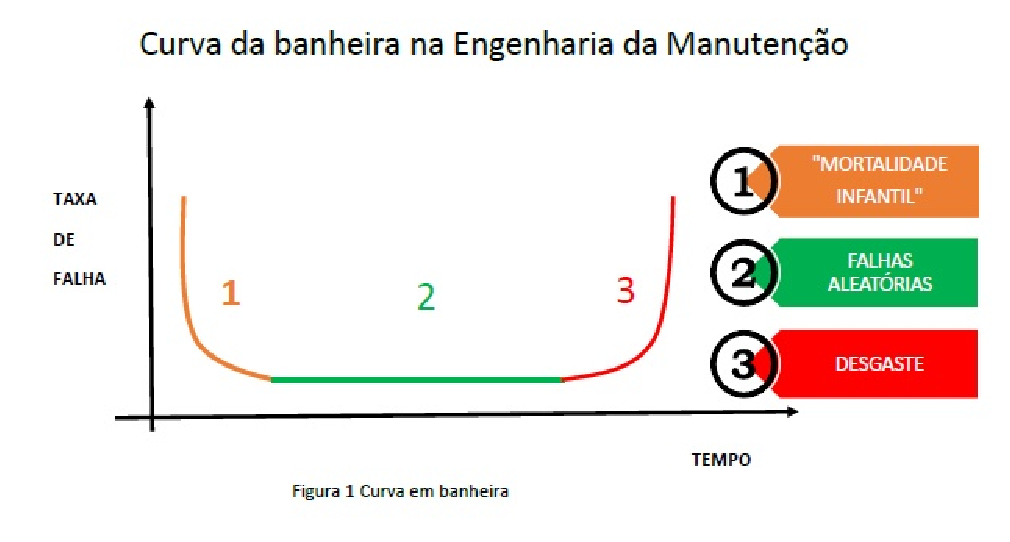
\includegraphics[width=0.8\textwidth]{curva_da_banheira.eps}
\caption{Teoria da curva da banheira \textbf{Fonte:A Curva da Banheira na Engenharia da Manutenção:2016.}}
\label{Curva da banheira}
\end{figure}

Conforme observado no gráfico acima, as frequências de ocorrência das falhas em um equipamento podem ser classificadas em 1) decrescente; 2) constante ou aleatória e 3) crescente, estando associadas ao estágio do ciclo de vida do equipamento.

\begin{itemize}
	\item \textbf{1) Decrescente:} Nesta fase, também denominada de \lq\lq mortalidade infantil \rq\rq, ocorrem falhas advindas dos defeitos de projeto, de fabricação e de instalação. É caracterizada por uma alta taxa de falha no início de sua operação;
	\item \textbf{2) Constante ou aleatória:} Esta fase costuma ser denominada de vida normal ou fase de estabilidade do equipamento, uma vez que a taxa de falhas é aproximadamente constante e ocorrem aleatoriamente, estando associadas a aplicação de esforços acidentais e/ou erros de manutenção. A taxa de falha é menor do que nas demais fases;
	\item \textbf{3) Crescente:} Esta fase reflete o período de instabilidade próprio do fim da vida útil do equipamento, ou seja, o sistema e seus componentes apresentam falhas por desgaste natural, decorrente do seu uso. Há um aumento considerável da taxa de falha nesta fase.  
\end{itemize} 

O conhecimento da \lq\lq curva da banheira \rq\rq por parte das instituições auxilia no controle da manutenção, na determinação da vida útil, no estabelecimento do tempo de garantia e na adoção de medidas indispensáveis para o aumento da disponibilidade e confiabilidade dos equipamentos.

Koren e Krishna \cite{koren2007} dizem em seu livro \emph{Fault-Tolerant System} que todo tipo de tolerância a falhas é um exercício de explorar e gerenciar redundância. Redundância é a propriedade de ter mais de um recurso do que o minimamente necessário para o trabalho sendo feito. Quando acontece uma falha, a redundância é explorada par mascarar ou contornar essas falhas, mantendo o nível desejado de funcionalidade. Eles trazem quatro tipos de redundância: de hardware, de software, de informação e de tempo. Abaixo será relatado como os autores tratam os conceitos relacionados a \textbf{tolerância a falhas}. 

A tolerância a falhas tem como objetivo tornar máquinas mais confiáveis, por isso ela tem medidas próprias. Medida é uma abstração matemática, que expressa uma observação da performance de um objeto. O truque em definir medidas adequadas é manter o subsistema largo o suficiente para que o comportamento de interesse do usuário seja capturado, e ainda assim não tão largo, para que a medida não perca o foco. 

\section{Modelagem da falha de equipamentos eletrônicos}

Embora a maioria das causas que levam os equipamentos ao desgaste estejam ligadas a seu uso, eventualmente, podem ter ocorrido problemas durante o seu processo de fabricação, ocasionando a produção de componentes fora da especificação e mais frágeis. Estes equipamentos quais provavelmente irão apresentar problemas prematuros, quando colocados em operação. De acordo com Sanches (2010, p. 19) os equipamentos que apresentam defeitos/falhas provenientes dos processos de fabricação apresentam problemas em um período inicial, que em média corresponde à 5\% da sua vida útil – período conhecido como falhas prematuras ou precoces.

Ou quando se deseja melhorar as suas condições de uso, algumas delas estão relacionadas à escolha do equipamento mais indicado, ou quais modificações serão necessárias a serem feitas na infra-estrutura para adequadamente utilizá-lo.

Restabelecer características construtivas originais dos equipamentos, garantindo a eles um nível de desempenho esperado através da manutenção. 
Estas ações de correição e prevenção quando adotadas aumentam a eficiência operacional e o tempo de vida útil dos ativos da organização. 

